\documentclass[12pt, a4paper]{article}
\title{Петля гистерезиса (динамический метод) (3.4.5)}
\author{Стеценко Георгий, Б02-312}
\date{}
% !TeX encoding = UTF-8

\usepackage{geometry}
\usepackage{amsmath, amsfonts, amssymb, amsthm} % стандартный набор AMS-пакетов для математ. текстов
\usepackage{mathtext}
\usepackage[utf8]{inputenc} % кодировка utf8
\usepackage[russian]{babel} % русский язык
\usepackage[pdftex,dvipsnames]{xcolor} % работа с цветами
\usepackage[pdftex]{graphicx} % графика (картинки)
\usepackage{tikz,pgfplots} % рисунки
\usepackage{indentfirst}
%\usepackage[labelfont=bf,labelsep=endash,skip=3pt]{caption} % подпись картинок
% \usepackage{fancyhdr,pageslts} % настройка колонтитулов
\usepackage{enumitem} % работа со списками
\usepackage{floatrow,multicol,multirow,longtable,hhline} % работа с таблицами
\usepackage{float,wrapfig} % плавающие объекты
\usepackage{tcolorbox} % рамка вокруг текста
%\usepackage[calc]{datetime2} % дата
\usepackage{bm} % жирное начертание в формулах
\usepackage{physics} % физический пакет
\DeclareMathAlphabet\mathbfcal{OMS}{cmsy}{b}{n}
\usepackage{pgfornament} % красивые рюшечки и вензеля
\usepackage{mdframed}
\usepackage{derivative}
\usepackage{mathrsfs} %EDS
\usepackage{soul} % strikethorugh
%\usepackage{boondox-cal}

% ----------------------------------------
% Настройка шрифта

% Просто закооментируйте следующую строчку, если не работает. Будет другой шрифт, правда :(
% \usepackage{pscyr}

% ----------------------------------------
% Стилевые настройки

\usepackage{boldline} % жирная линия после таблиц (чтобы не было ошибок, этот пакет должен подключаться именно тут!)
\floatsetup[table]{style=Plaintop,floatrowsep=qquad} % настройка оформления таблиц
\setlist[enumerate,itemize]{leftmargin=5mm,itemindent=10mm,itemsep=0mm,
listparindent=0em,labelsep=2mm,topsep=2mm,labelwidth=4mm} % настройки списков

\setlength{\columnsep}{0.5cm} % расстояние между колонками
\setlength{\parskip}{1pt} % расстояние до текста от колонтитула

%\usepackage{titlesec} % управление оформлением section
%\renewcommand{\thesection}{\Roman{section}}
%\titleformat{\section}[block]{\bfseries\large}{\thesection.}{5pt}{}

% ----------------------------------------
% Настройки полей
\geometry{
  left=10mm,
  top=10mm,
  right=10mm,
  bottom=15mm,
  marginparsep=0mm,
  marginparwidth=0mm,
  headheight=0pt,
  headsep=0pt,
footskip=20pt}

% ----------------------------------------
% Настройки колонтитулов и нумерации страниц
\pagenumbering{arabic}



\newcounter{ntask}
\setcounter{ntask}{0}


\newcommand{\arsh}{\mathrm{arsh} \,\,}
\newcommand{\arch}{\mathrm{arch} \,\,}
\newcommand{\arth}{\mathrm{arth} \,\,}
\newcommand{\arcth}{\mathrm{arcth} \,\,}
\renewcommand{\Re}{\operatorname{Re} \,}
\newcommand{\EDS}{\mathscr{E}}
\newcommand{\diffract}[1]{\frac{\mathrm{d}#1}{\mathrm{d}t}}



\newcommand{\V}{~\mathrm{V}}
\newcommand{\mV}{~\mathrm{mV}}
\newcommand{\A}{~\mathrm{A}}
\newcommand{\mA}{~\mathrm{mA}}
\newcommand{\uT}{~\mathrm{\mu T}}
\newcommand{\mT}{~\mathrm{mT}}

\addto\captionsrussian{\def\refname{Источники}}

\begin{document}
\maketitle

\section{Цель работы}
Изучение петель гистерезиса различных ферромагнитных материалов в переменных полях.

\section{Теоретические сведения}
Магнитная индукция $B$ и напряжённость поля $H$ в ферромагнитном материале неоднозначно связаны между собой: индукция зависит не только от напряжённости, но и от предыстории образца. Связь между $B$ и $H$ типичного ферромагнетика иллюстрирует рисунок \ref{Theor}.

\begin{wrapfigure}[11]{r}{5.0cm}\vspace{-6mm}
  \centering
  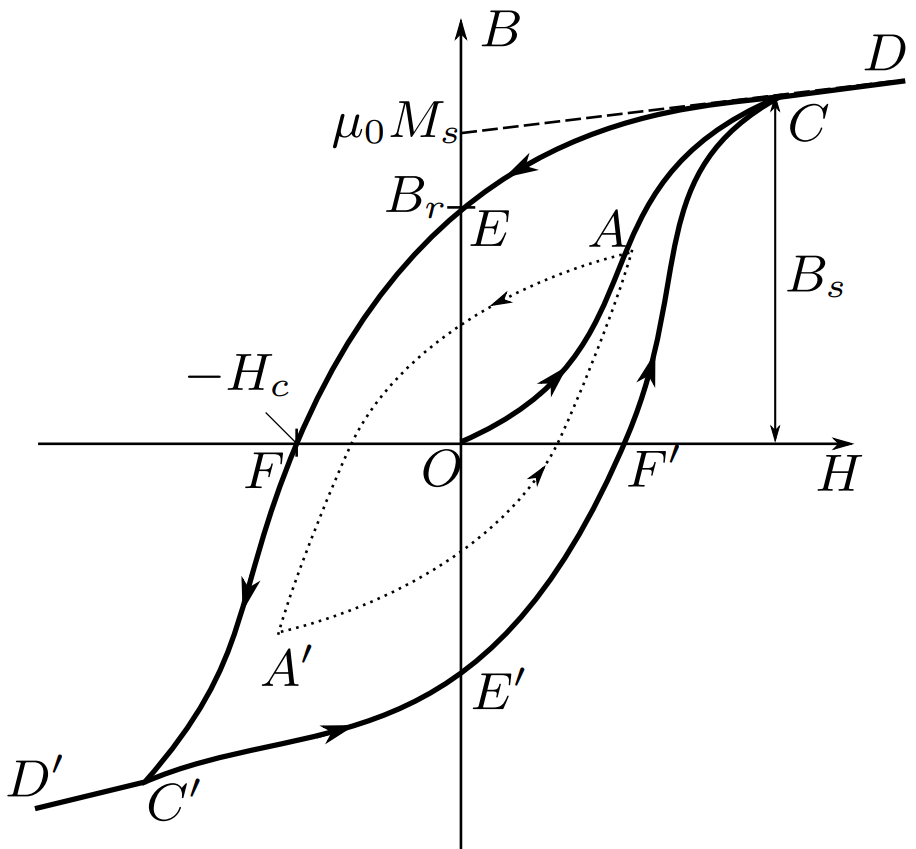
\includegraphics[width=4.5cm]{pics/Theor}
  \caption{Теоретический вид петли гистерезиса.}
  \label{Theor}
\end{wrapfigure}

Если к ферромагнитному образцу прикладывать переменное внешнее магнитное поле, то~его состояние на плоскости $H-B$ будет изменяться по замкнутой кривой~-- \textit{петле гистерезиса}.
Резмер петли определяется максимальным значением напряжённости $H$ в цикле (например, петля $AA'$, обозначенная пунктиром на рисунке \ref{Theor}).
Если амплитуда напряжённости достаточно велика, то образец будет периодически достигать \textit{насыщения},
что на рисунке \ref{Theor} соответствует кривой $CERC'E'F'C$ (\textit{предельная петля гистерезиса}).
Пересечение предельной петли~с вертикальной осью соответствует остаточной индукции $B_r$, пересечение~с горизонтальной осью -- коэрцитивному полю $H_c$.
Крайние точки петель, соответствующие амплитудным значениям $H$ (например, точка $A$ на рисунке \ref{Theor}), лежат на \textit{начальной кривой намагничивания} ($OAC$).

\textbf{Измерение магнитной индукции.} Магнитную индукцию $B$ удобно определять с~помощью ЭДС, возникающей при измерении магнитного потока $\Phi$ в катушке, намотанной на образец. Пусть катушка с $N$ витками плотно охватывает образец сечением $S$, и индукция $B$ в образце однородна. Тогда\[\left|B\right|=\frac{1}{SN}\int\EDS\text{d}t.\]Таким образом, для определения $B$ нужно проинтегрировать сигнал, наведённый меняющимся магнитным полем в измерительной катушке, намотанной на образец.

Для интегрирования в работе используется \textit{интегрирующая RC-цепочка}.
Входное напряжение от источника $U_{\text{вх}}(t)$ подаётся на последовательно соединённые резистор $R_{\text{и}}$ и конденсатор $C_{\text{и}}$.
Выходное напряжение $U_{\text{вых}}(t)$ снимается с~конденсатора.
Предположим, что (1) сопротивление источника мало по сравнению с~$R_{\text{и}}$;
(2) выходное сопротивление (сопротивление на входе осциллографа), напротив, велико:
$R_{\text{вых}}\gg R_{\text{и}}$; и, наконец, (3) сопротивление $R_{\text{и}}$ достаточно велико,
так что почти всё падение напряжения приходится на него, а $U_{\text{вых}}\ll U_{\text{вх}}$.
В~таком случае ток цепи равен $I=\frac{U_{\text{вх}}-U_{\text{вых}}}{R_{\text{и}}}\approx\frac{U_{\text{вх}}}{R_{\text{и}}}$,
и входное и выходное сопротивление связаны соотношением\[U_{\text{вых}}\frac{q}{C_{\text{и}}}=\frac{1}{C_{\text{и}}}\int_0^tI\text{d}t\approx\frac{1}{\tau_{\text{и}}}\int_0^tU_{\text{вх}}\text{d}t,\]где $\tau_{\text{и}}=R_{\text{и}}C_{\text{и}}$ -- постоянная времени $RC$-цепочки.
Для индукции поля получаем\[\left|B\right|=\frac{1}{SN}\int U_{\text{вх}}\text{d}t=\frac{\tau_{\text{и}}}{SN}U_{\text{вх}}.\]

Уточним, когда наше предположение справедливо. Необходимо, чтобы было выполнено \[U_\text{вых} / U_\text{вх} = \frac{\frac{1}{\omega C_\text{и}}}{\sqrt{R_\text{и}^2 + \frac{1}{\omega^2 C_\text{и}^2}}},\]
то есть $R \gg \frac{1}{\omega C}$, что равносильно $\tau_\text{и} = R_\text{и}C_\text{и} \gg \frac{1}{\omega}$ (характерное время релаксации много больше периода вынужденных колебаний).

\section{Методика измерений и результаты}
\textbf{В~работе используются:} автотрансформатор, понижающий трансформатор,
интегрирующая цепочка, амперметр, вольтметр, электронный осциллограф, делитель напряжения,
тороидальные образцы с~двумя об­мотками.

\begin{figure}[H]
  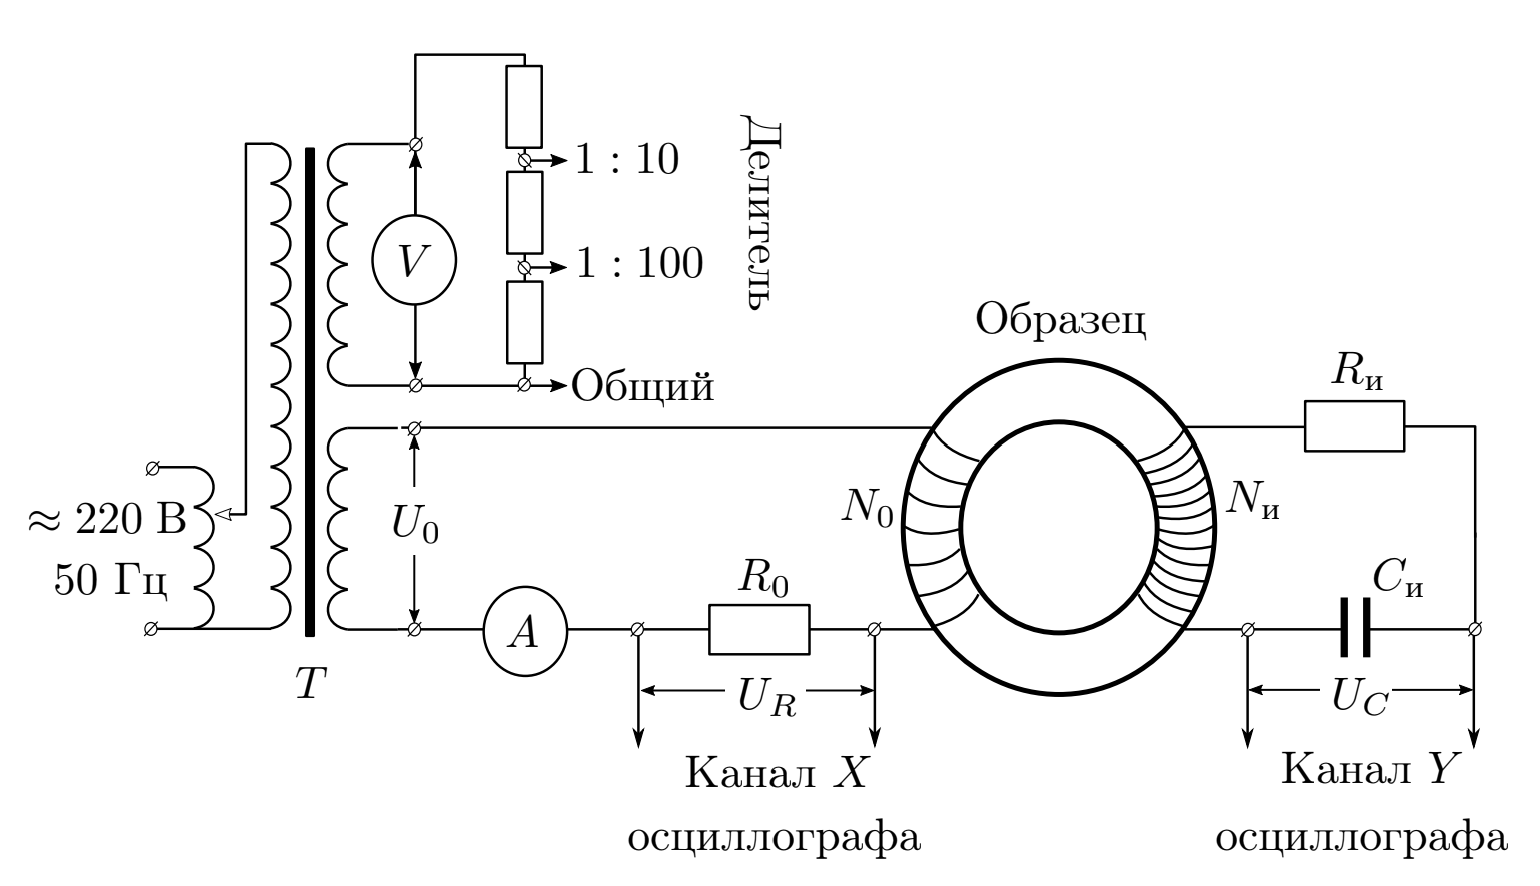
\includegraphics[width=0.8\linewidth]{pics/setup.png}
  \caption{Схема установки}
  \label{pic_setup}
\end{figure}

Пользуясь уравнениями Максвелла, поймём, как в нашей работе связаны мгновенные значения напряжений с индукцией и напряжённостью
магнитного поля.
\begin{equation}
  H = \frac{N_0 U_R}{R_0 \cdot 2\pi R}
  \label{eq:H}
\end{equation}
\begin{equation}
  B = \frac{R_\text{и}C_\text{и} U_C}{ N_\text{и} S}
  \label{eq:B}
\end{equation}
\subsection{Подготовка. Проверка калибровки осциллографа}
\textbf{Горизонтальная ось.} Здесь контакты, которые шли на намагничивающий контур $N_0$ закорачиваются.
При масштабе клетки в $10\mV$ действующему значению тока в $56.12\mA$ через резистор
$R_0 = 0.3~\Omega$ соответствовал размах на осциллографе, равный $5.0$ клеткам.
\[I^\text{д}_{osc} = \frac{50\mV}{2\cdot 0.3~\Omega} \cdot \frac{1}{\sqrt 2} = 58.9 \mA,\]
что достаточно хорошо совпадает с измеренным на амперметре действующим значением. Корректировка значений с осциллографа не требуется.

\textbf{Вертикальная ось.} Здесь измерение происходит в калибровочном контуре (верхняя вторичная обмотка на трансформаторе $T$).
При масштабе клетки в $50\mV$ действующему значению напряжения в $13.5\V$ на калибровочном делителе
1:100 соответствовал размах на осциллографе, равный $7.8$ клеткам.
\[U^\text{д}_{osc} = {7.8\cdot 50\mV} \cdot 100\cdot  \frac{1}{\sqrt 2} = 13.8 \V,\]
что достаточно хорошо совпадает с измеренным на вольтметра действующим значением. Корректировка значений с осциллографа не требуется.

\subsection{Подготовка. Проверка предположения о линейности переходной характеристики интегрирующей цепи}
Подадим на участок RC переменное напряжение, и снимем показания напряжения на всём участке и только на конденсаторе.
$2 U_\text{C.m} = 7.6 \cdot 20 \mV = 152 \mV$, $2U_\text{RC.m} = 3.8* 5 \V = 19 \V$, ${\frac{Z_\text{C}}{Z_\text{CR}} \approx \frac{1}{\omega \cdot CR} \approx 0.8 \% \ll 1}$.
Значит, наше предположение выполнено, и CR-делитель действительно можно считать интегрирующей цепочкой.

\subsection{Петля гистерезиса на экране осциллографа}
На рис. \ref{pic_setup} изображена схема экспериментальной установки.
Напряжение с латра, работающего в диапазоне $0\sim250\V$, понижается на трансформаторе $T$
и подаётся на контур с исследуемой катушкой. Ток в первичной обмотке, пропорциональный напряженности магнитного поля, измеряется
токоизмерительным резистором $R_0$, а интеграл ЭДС индукции во вторичной обмотке, пропорциональное индукции магнитного поля,
измеряется по величине напряжения на конденсатора $C_и$ в интегрирующей цепочке.

Перечислим свойства исследуемых катушек:
\begin{table}[H]
  \centering
  \begin{tabular}{|c|c|c|c|c|}
    \hline
    Материал     & $N_0$ & $N_\text{и}$ & $S^2$, см$^2$ & $2\pi R$, см \\ \hline
    Феррит       & 35    & 400                              & 3.0           & 25         \\ \hline
    Пермаллой    & 40    & 200                              & 3.8           & 24         \\ \hline
    Крем. железо & 25    & 250                              & 2.0           & 11         \\ \hline
  \end{tabular}
  \caption{Характеристики катушек}
  \label{tab:har_kat}
\end{table}

Снимем предельные петли гистерезиса и будем медленно их уменьшать, чтобы по концам петель восстановить кривую намагничивания.
Результаты измерений приведены в векторизированном виде на рис. \ref{fig:curves}.

\begin{figure}[H]
  \begin{minipage}{.33\textwidth}
    \centering
    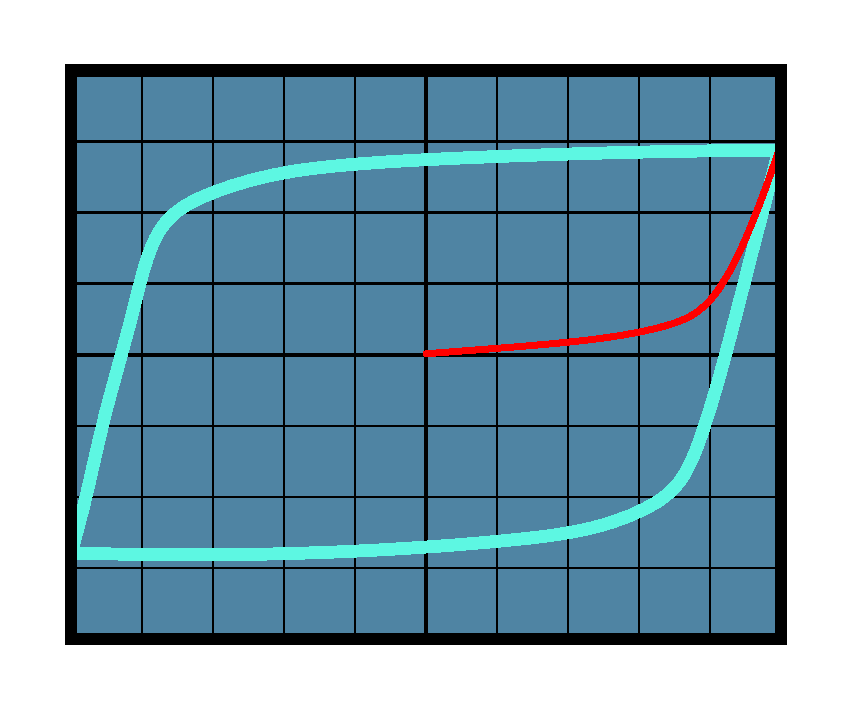
\includegraphics[width=.95\linewidth]{pics/permalloy.pdf}
  \end{minipage}%
  \begin{minipage}{.33\textwidth}
    \centering
    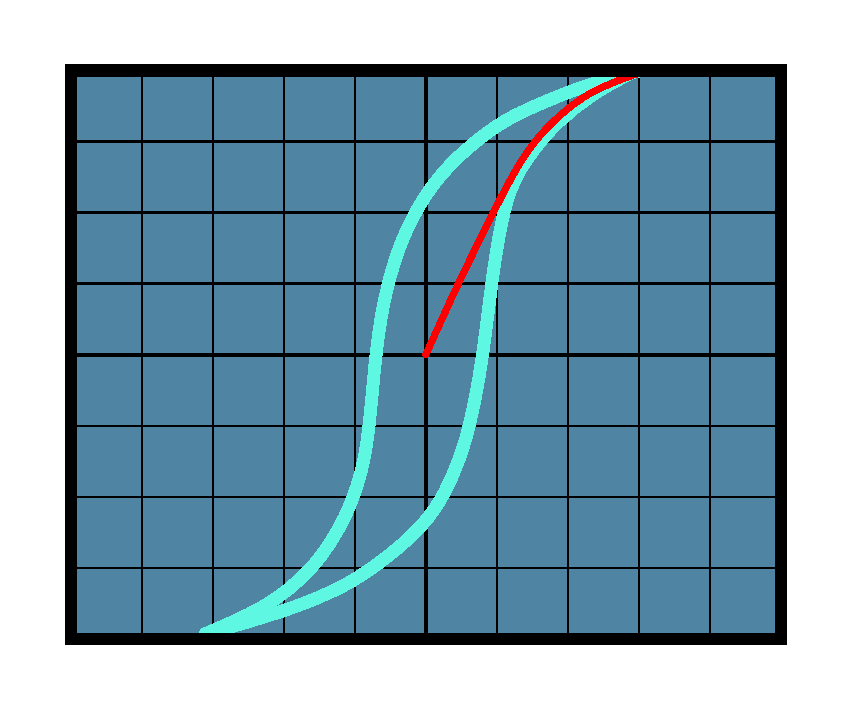
\includegraphics[width=.95\linewidth]{pics/FeSi.pdf}
  \end{minipage}%
  \begin{minipage}{.33\textwidth}
    \centering
    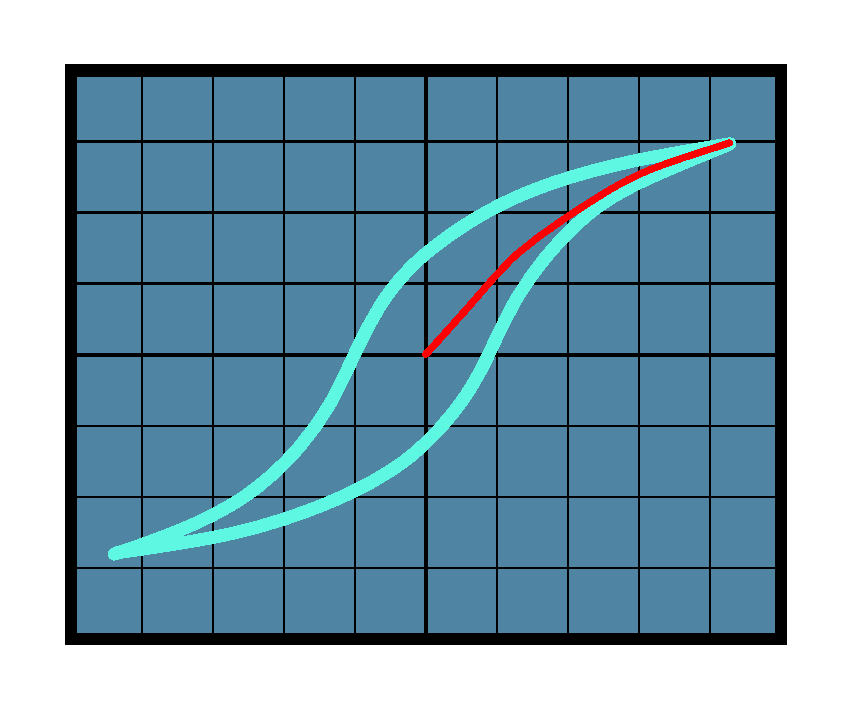
\includegraphics[width=.95\linewidth]{pics/Ferrit.pdf}
  \end{minipage}
  \centering
  \caption{\centering Кривые гистерезиса (зелёным цветом) и криывые намагничивания (красным). Слева~направо: пермаллой, кремнистое железо, феррит}
  \label{fig:curves}
\end{figure}

Видно, что была допущена ошибка при измерении для пермаллоя: начальная кривая намагничивания не выходит на насыщение.
Это означает, что была снята не предельаня петля гистерезиса, а одна из меньших. Тем не менее, дифференциальную магнитную проницаемость
всё ещё можно измерить.

Пользуясь соотношениями (\ref{eq:H}) и (\ref{eq:B}), пересчитаем масштаб по осям для каждой катушки:
\begin{table}[H]
  \centering
  \begin{tabular}{|c|c|c|c|c|}
    \hline
    Материал      & $K_x, \mathrm{mV/div}$
    & $K_y, \mathrm{mV/div}$
    & $B_0$, $\mathrm{mT/div}$
    & $H_0$, $\mathrm{A/m/div}$ \\ \hline
    Пермаллой     & 10 & 50 & 52.6 & 11.1     \\ \hline
    Крем. железо  & 20 & 10 & 80.0 & 15.2     \\ \hline
    Феррит        & 50 & 50 & 167  & 23.3     \\ \hline
  \end{tabular}
  \caption{Коэффициенты усиления}
  \label{tab:ampl_cefs}
\end{table}

Тогда по графикам найдём и искомые величины:
\begin{table}[H]
  \centering
  \begin{tabular}{|c|c|c|c|c|}
    \hline
    Материал      & $Н_с,~\mathrm{A/m}$
    & $B_r, \mathrm{mT}$
    & $\mu _\text{dif}^{max}$, $\mathrm{1}$
    & $B_s, \mathrm{mT}$ \\ \hline
    Пермаллой     & -- & -- & 9800 &   --    \\ \hline
    Крем. железо  & 12 & 184 & 8800 &  360    \\ \hline
    Феррит        & 21 & 220 & 6300 &  580    \\ \hline
  \end{tabular}
  \caption{Полученные характеристики сплавов}
  \label{tab:chars}
\end{table}


\section{Обсуждение результатов и вывод}
Были получены кривые гистерезиса для катушек из трёх различных материалов. 
Для них так же были построены кривые начального намагничивания. В ходе обработки обнаружилось, 
что для одного из образцов точно была снята характеристика, далёкая от предельной. Тем не менее,
была показана возможность пользоваться описанной схемой для построения петли гистерезиса в реальном времени
и получены некоторые численные результаты, которые хоть и достаточно далеки от табличных, 
всё же близки к ним по порядку. 

\end{document}
